%%%%%%%% ICML 2019 EXAMPLE LATEX SUBMISSION FILE %%%%%%%%%%%%%%%%%

\documentclass{article}

% Recommended, but optional, packages for figures and better typesetting:
\usepackage{microtype}
\usepackage{graphicx}
\usepackage{subfigure}
\usepackage{booktabs} % for professional tables

% hyperref makes hyperlinks in the resulting PDF.
% If your build breaks (sometimes temporarily if a hyperlink spans a page)
% please comment out the following usepackage line and replace
% \usepackage{icml2019} with \usepackage[nohyperref]{icml2019} above.
\usepackage{hyperref}

% Attempt to make hyperref and algorithmic work together better:
\newcommand{\theHalgorithm}{\arabic{algorithm}}

% Use the following line for the initial blind version submitted for review:
\usepackage{icml2019}

% If accepted, instead use the following line for the camera-ready submission:
%\usepackage[accepted]{icml2019}

% The \icmltitle you define below is probably too long as a header.
% Therefore, a short form for the running title is supplied here:
\icmltitlerunning{Submission and Formatting Instructions for ICML 2019}

\begin{document}

\twocolumn[
\icmltitle{Submission and Formatting Instructions for \\
           International Conference on Machine Learning (ICML 2019)}

% It is OKAY to include author information, even for blind
% submissions: the style file will automatically remove it for you
% unless you've provided the [accepted] option to the icml2019
% package.

% List of affiliations: The first argument should be a (short)
% identifier you will use later to specify author affiliations
% Academic affiliations should list Department, University, City, Region, Country
% Industry affiliations should list Company, City, Region, Country

% You can specify symbols, otherwise they are numbered in order.
% Ideally, you should not use this facility. Affiliations will be numbered
% in order of appearance and this is the preferred way.
\icmlsetsymbol{equal}{*}

\begin{icmlauthorlist}
\icmlauthor{Aeiau Zzzz}{equal,to}
\icmlauthor{Bauiu C.~Yyyy}{equal,to,goo}
\icmlauthor{Cieua Vvvvv}{goo}
\icmlauthor{Iaesut Saoeu}{ed}
\icmlauthor{Fiuea Rrrr}{to}
\icmlauthor{Tateu H.~Yasehe}{ed,to,goo}
\icmlauthor{Aaoeu Iasoh}{goo}
\icmlauthor{Buiui Eueu}{ed}
\icmlauthor{Aeuia Zzzz}{ed}
\icmlauthor{Bieea C.~Yyyy}{to,goo}
\icmlauthor{Teoau Xxxx}{ed}
\icmlauthor{Eee Pppp}{ed}
\end{icmlauthorlist}

\icmlaffiliation{to}{Department of Computation, University of Torontoland, Torontoland, Canada}
\icmlaffiliation{goo}{Googol ShallowMind, New London, Michigan, USA}
\icmlaffiliation{ed}{School of Computation, University of Edenborrow, Edenborrow, United Kingdom}

\icmlcorrespondingauthor{Cieua Vvvvv}{c.vvvvv@googol.com}
\icmlcorrespondingauthor{Eee Pppp}{ep@eden.co.uk}

% You may provide any keywords that you
% find helpful for describing your paper; these are used to populate
% the "keywords" metadata in the PDF but will not be shown in the document
\icmlkeywords{Machine Learning, ICML}

\vskip 0.3in
]

% this must go after the closing bracket ] following \twocolumn[ ...

% This command actually creates the footnote in the first column
% listing the affiliations and the copyright notice.
% The command takes one argument, which is text to display at the start of the footnote.
% The \icmlEqualContribution command is standard text for equal contribution.
% Remove it (just {}) if you do not need this facility.

%\printAffiliationsAndNotice{}  % leave blank if no need to mention equal contribution
\printAffiliationsAndNotice{\icmlEqualContribution} % otherwise use the standard text.

\begin{abstract}
Recent latent semantics analysis are based on calculating the word vector distance between target and goal sentences or proposing generalized semantic hypothesis according to the original text. In this project, we explore the higher level mission on challenging one of the COPA task which is analysing common sense from ordinary scenario description text. We successfully boost our BERT model performance with test accuracy of 78\% among IBM research AI, BERT-mtl model with accuracy of 73.8\% on the SuperGlue leaderboard 2.0. During the enhancement of model, we conjecture that the key factors in model performance is that (1) The word embedding format. (2) The scale of our fine tuning data. (3) The configuration of BERT model Introduction. We demonstrated the potential of BERT model. Experiments shows new state-of-the-art of BERT model results on COPA without any bells and whistles.  
\end{abstract}



\section{Introduction}

\label{submission}
The motivation of this project is to analyze the common sense from choice of plausible alternatives where each question is composed of a premise and two alternatives, and the task is to select the alternative that more plausibly has a causal relation with the premise. Here’s the data format:
\begin{center}
\begin{itemize}
    \item \textbf{Premise}: The item was packaged in bubble wrap.
    \item \textbf{Alternative1}: It was fragile.
    \item \textbf{Alternative2}: It was small.
    \item \textbf{Question type}: Cause
    \item \textbf{Label}: Alternative1
\end{itemize}
\end{center}
The milestones below will show how we studied the COPA data and how we get the reasonable prediction based on the data format:
\begin{itemize}
\item Calculating Manhattan distance between premises and complete sentences.  
\item Using BERT model to calculate the euclidean distance between sentences.
\end{itemize}

\subsection{Siamese Manhattan LSTM}

\textbf{Manhattan LSTM models} has two networks $LSTM_{left}$ and $LSTM_{right}$ which process one of the sentences in a given pair independently. And a version of Manhattan LSTM where both $LSTM_{left}$ and $LSTM_{right}$ have same tied weights such that $LSTM_{left} = LSTM_{right}$. The model uses an LSTM to read in word-vectors representing each input sentence and employs its final hidden state as a vector representation for each sentence. Subsequently, the similarity between these representations is used as a predictor of semantic similarity.

\begin{figure}[ht]
\vskip 0.2in
\begin{center}
\centerline{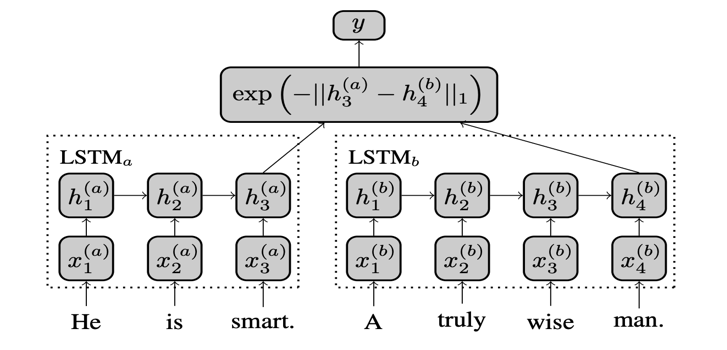
\includegraphics[width=\columnwidth]{Picture1.png}}
\caption{Siamese Manhattan LSTM}
\label{icml-historical}
\end{center}
\vskip -0.2in
\end{figure}
Here's our initial thought on how to use Siamese Manhattan LSTM model.
\begin{itemize}
    \item Instead of initializing the Siamese networks on our test data (500 questions combined with two answers for each) to directly calculate distance between query and answer, we decide to pre-train the Siamese Manhattan LSTM with SICK data which contains 9,927 sentence pairs with a $5,000/4,927$ training/test split ( Each pair is annotated with a relatedness $label \in [1, 5]$ corresponding to the average relatedness judged by 10 different individuals).
    \item Then we would use our Siamese Manhattan LSTM trained from step 1 as our classifier to calculate the Manhattan distance between each query with their corresponding answer.
    \item We would pre-process our data based on cause & effect model, which means we would combine question and answer according to the model as our new data format, then we compare the two options in one query: \\
     $If \ Condition = cause,data1 = query1 + answer1, data2 = query1 + answer 2$ \\
    $If \ Condition = effect, data1 = answer1 + query1, data2 = answer2 + query2$
    \item The Loss can be conclude into three part $loss_{pretrained model}, 
    loss_{SimilarityCalculation}$ and $loss_{Classification}$
\end{itemize}

\textbf{Discussion:} According to our research on the Manhattan LSTM model, we observe the Manhattan LSTM model only works with naive similarity comparisons without analyzing the deep level of latent semantics meaning. Directly calculate and compare the word embedding vector distance through siames structure model is not capable for the LSTM network to obtain thorough comprehension on common sense from the COPA data.


\subsection{BERT}

\textbf{Bidirectional Encoder Representations from Transformers}
makes use of Transformer, an attention mechanism that learns contextual relations between words (or sub-words) in a text. In its vanilla form, Transformer includes two separate mechanisms — an encoder that reads the text input and a decoder that produces a prediction for the task. BERT learning model(LM) has obtained new state-of-the-art results on eleven natural language processing tasks, including the GLUE and SuperGLUE benchmarks.  Currently 5 of the top scores on the SuperGLUE leaderboard are using BERT based models.Our team proposes to use the opensource BERT pre-training language model as the basis of our implementation for the COPA task.
\\
There are two steps to the BERT model: pre-training and fine-tuning. During pre-training, the model is trained on unlabeled data over different pre-training tasks. For fine-tuning, the BERT model is first initialized with the pre-trained parameters, and all of the parameters are fine-tuned using labeled data from the downstream tasks.
\begin{figure}[ht]
\vskip 0.2in
\begin{center}
\centerline{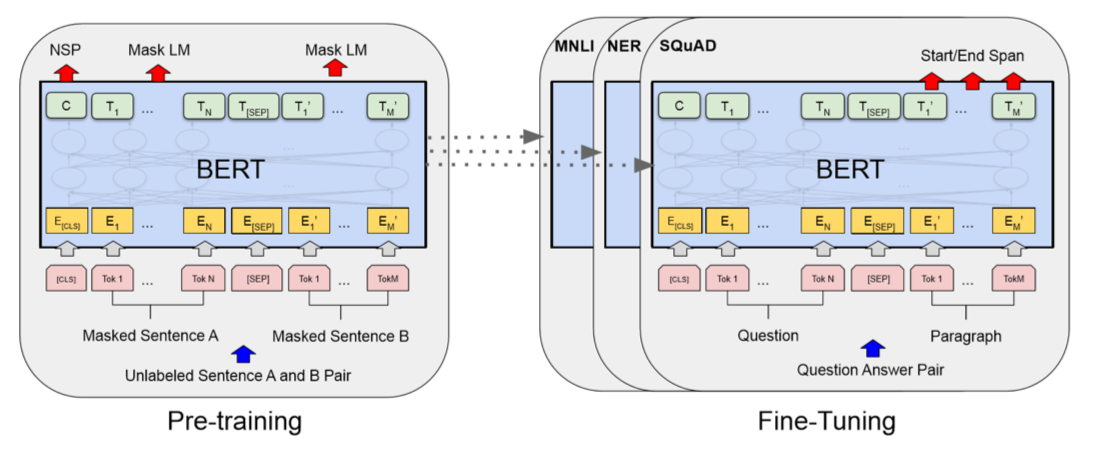
\includegraphics[width=\columnwidth]{BERT.png}}
\caption{BERT}
\label{icml-historical}
\end{center}
\vskip -0.2in
\end{figure}

\begin{itemize}

    \item As stated before, the COPA task provides a training dataset of 400 examples and evaluation dataset of 100 examples
    
    \item We are generating new COPA training data by taking the MultiNLI training data, from the original GLUE task, and creating new COPA examples.  The MultiNLI training set has over 10,000 examples.
    \item \textbf{MultiNLI to COPA:}
    $$Entailment$$
    $$COPA \ premise = initial \ sentence$$
    $$ COPA \ Alternative1 = entitled \ sentence $$
    $$ COPA \ Alternative2 = neutral \ sentence $$
    $$   COPA \ Choice = Alternative1 $$
    $$Neutral$$
    $$ COPA \ Alternative1 = entitled \ sentence $$
    $$ COPA \ Alternative2 = contradiction \ sentence $$
    $$   COPA \ Choice = Alternative1 $$
    $$Contradiction$$
    $$ COPA \ Alternative1 = contradiction \ sentence $$
    $$ COPA \ Alternative2 = neutral \ sentence $$
    $$   COPA \ Choice = Alternative2 $$
    
    \item We will pre-process our data similar to how we would for the Siamese LSTM model, except this time we will add [CLS] to the start of the data field, and use [SEP] to separate the premise and the possible cause & effects. \\ 
    $$Condition = cause$$
    $$data1 = [CLS]query1 [SEP] answer1$$
    $$data2 = [CLS]query1 [SEP] answer 2$$

    \item BERT will create an contextual aware embedding vector for each word part in the two sentences.  It will also create a embedding value for the tokens [CLS] and [SEP] which is based on sentence level embedding
    \item We then calculate the Euclidean distance between the embedded vectors for the word parts in the two sentences.  We also calculate Cosine similarity between the [CLS] and [SEP] sentence level embedding.
    \item We would select the answer that minimizes these values.
\end{itemize}
\section{Data exploration}
Since Our initial BERT model got 64\% training accuracy with batch size=5 and epoch = 10. However, the accuracy reduced after increasing the training epochs. After observing the data, we decide to attempt to classify the data with an additional label.  The label allows us to separate or data into two sets called “hard data” and “easy data”.  We did this by manually pre-processing the training data.

\textbf{Case 1:}\\
P:  The man got a discount on his groceries. \\ A1: He greeted the cashier.\\ A2: He used a coupon \\
\textbf{Step 1:}Remove all stop words: the, a, on, his, he.
\\
P:   man, got, discount, groceries. \\
A1: greeted, cashier. \\ 
A2: used, coupon. \\
\textbf{Step 2:}Any pair words?   \textbf{Yes, (Discount—Coupon)}
\\
\textbf{Step 3:} Does the number of similar words $>=50 \%$?   \textbf{No}\\
\textbf{Step 4:} Label 0 (Easy)

\textbf{Case 2:}\\
P:  The heavyset man decided to lose weight.
 \\ A1: He cut out sweets.
\\ A2: He avoided caffeine. \\
\textbf{Step 1:}Remove all stop words: the, to, out, he. 
\\
P:   heavyset, man, decided, lose, weight. \\
A1: cut, sweets. \\ 
A2: avoided, caffeine. \\
\textbf{Step 2:}Any pair words?   \textbf{No}
\\
\textbf{Step 3:} Label 1 (Difficult)

\textbf{Case 3:}\\
P:I deposited the letter in the mailbox.
 \\ A1: The post office delivered the letter.
\\ A2: The post office expedited the letter.
 \\
\textbf{Step 1:}Remove all stop words: I, the, in.
\\
P: deposited, letter, mailbox.
 \\
A1: post, office, delivered, letter. \\ 
A2: post, office, expedited, letter. \\
\textbf{Step 2:}Any pair words? \\  \textbf{Yes,(mailbox—letter)(mailbox—post, office)}
\\
\textbf{Step 3:} Does the number of similar words $>=50 \%$?   \textbf{Yes}\\
\textbf{Step 4:} Label 1 (Difficult)

\begin{algorithm}[tb]
   \caption{Sentence selection}
   \label{alg:example}
\begin{algorithmic}
   \STATE {\bfseries Input:} Premise $P_i$, Alternative1 $A_1$, Alternative2 $A_2$, Data Amount $N$
   \REPEAT
   \STATE Initialize $Label = [\ ]$.
   \FOR{$i=1$ {\bfseries to} $N-1$}
   \IF{$There\ are\ any\ pair\ words\ and\ Number\ of\ similar\ word>50 \% $}
  \STATE $Label.append(1(Difficult))$
   \ELSIF{$There\ are\ any\ pair\ words\ and\ Number\ of\ similar\ word<=50 \% $}
   \STATE $Label.append(0(Easy))$
   \ELSIF{$There\ are\ not\ any\ pair\ words\ $}
   \STATE $Label.append(1(Difficult))$
   \ENDIF
   \ENDIF
   \ENDFOR
\end{algorithmic}
\end{algorithm}
\subsection{Model performance}
After implementing data selection algorithm, we observe the model performance on each algorithm. 
\begin{table}[t]
\caption{Test accuracy on different type of training data}
\label{sample-table}
\vskip 0.15in
\begin{center}
\begin{small}
\begin{sc}
\begin{tabular}{lcccr}
\toprule
Model & Acc(Easy data) & Acc(difficult data)  \\
\midrule
Initial Bert    & 70\% & 55\% \\
Initial Roberta    & 64\% & 60\% \\
Second Roberta    & 67\% & 58\% \\
Our Bert        & 78\% & 64\% \\

\bottomrule
\end{tabular}
\end{sc}
\end{small}
\end{center}
\vskip -0.1in
\end{table}

Submitted papers can be up to eight pages long, not including references, and up to twelve pages when references and acknowledgments are included.
Acknowledgements should be limited to grants and people who contributed to the paper.
Any submission that exceeds
this page limit, or that diverges significantly from the specified format,
will be rejected without review.

The text of the paper should be formatted in two columns, with an
overall width of 6.75~inches, height of 9.0~inches, and 0.25~inches
between the columns. The left margin should be 0.75~inches and the top
margin 1.0~inch (2.54~cm). The right and bottom margins will depend on
whether you print on US letter or A4 paper, but all final versions
must be produced for US letter size.

The paper body should be set in 10~point type with a vertical spacing
of 11~points. Please use Times typeface throughout the text.


\section*{Acknowledgements}

\textbf{Do not} include acknowledgements in the initial version of
the paper submitted for blind review.

If a paper is accepted, the final camera-ready version can (and
probably should) include acknowledgements. In this case, please
place such acknowledgements in an unnumbered section at the
end of the paper. Typically, this will include thanks to reviewers
who gave useful comments, to colleagues who contributed to the ideas,
and to funding agencies and corporate sponsors that provided financial
support.


% In the unusual situation where you want a paper to appear in the
% references without citing it in the main text, use \nocite
\nocite{langley00}

\bibliography{example_paper}
\bibliographystyle{icml2019}


%%%%%%%%%%%%%%%%%%%%%%%%%%%%%%%%%%%%%%%%%%%%%%%%%%%%%%%%%%%%%%%%%%%%%%%%%%%%%%%
%%%%%%%%%%%%%%%%%%%%%%%%%%%%%%%%%%%%%%%%%%%%%%%%%%%%%%%%%%%%%%%%%%%%%%%%%%%%%%%
% DELETE THIS PART. DO NOT PLACE CONTENT AFTER THE REFERENCES!
%%%%%%%%%%%%%%%%%%%%%%%%%%%%%%%%%%%%%%%%%%%%%%%%%%%%%%%%%%%%%%%%%%%%%%%%%%%%%%%
%%%%%%%%%%%%%%%%%%%%%%%%%%%%%%%%%%%%%%%%%%%%%%%%%%%%%%%%%%%%%%%%%%%%%%%%%%%%%%%
\appendix
\section{Do \emph{not} have an appendix here}

\textbf{\emph{Do not put content after the references.}}
%
Put anything that you might normally include after the references in a separate
supplementary file.

We recommend that you build supplementary material in a separate document.
If you must create one PDF and cut it up, please be careful to use a tool that
doesn't alter the margins, and that doesn't aggressively rewrite the PDF file.
pdftk usually works fine. 

\textbf{Please do not use Apple's preview to cut off supplementary material.} In
previous years it has altered margins, and created headaches at the camera-ready
stage. 
%%%%%%%%%%%%%%%%%%%%%%%%%%%%%%%%%%%%%%%%%%%%%%%%%%%%%%%%%%%%%%%%%%%%%%%%%%%%%%%
%%%%%%%%%%%%%%%%%%%%%%%%%%%%%%%%%%%%%%%%%%%%%%%%%%%%%%%%%%%%%%%%%%%%%%%%%%%%%%%


\end{document}


% This document was modified from the file originally made available by
% Pat Langley and Andrea Danyluk for ICML-2K. This version was created
% by Iain Murray in 2018, and modified by Alexandre Bouchard in
% 2019. Previous contributors include Dan Roy, Lise Getoor and Tobias
% Scheffer, which was slightly modified from the 2010 version by
% Thorsten Joachims & Johannes Fuernkranz, slightly modified from the
% 2009 version by Kiri Wagstaff and Sam Roweis's 2008 version, which is
% slightly modified from Prasad Tadepalli's 2007 version which is a
% lightly changed version of the previous year's version by Andrew
% Moore, which was in turn edited from those of Kristian Kersting and
% Codrina Lauth. Alex Smola contributed to the algorithmic style files.
